\subsection{Amplifier Stage}

The current transducers output a $\pm \SI{25}{\milli\volt}$ signal centered around $\SI{2.5}{\volt}$.
This signal must be amplified to $\pm \SI{2.5}{\volt}$ using an operational amplifier with a gain of 100.
This amplified signal is then fed into the microcontroller's ADC input.
To realise this, we have used a non-inverting op-amp circuit (figure \ref{fig:non-inverting-op-amp}) for each signal.
The input impedance and gain for the non-inverting amplifier circuit are given by equations \ref{eq:zi} and \ref{eq:gain} respectively.
The half-rail voltage of $\SI{2.5}{\volt}$ is provided by a virtual ground op-amp circuit (figure \ref{fig:half-supply}).
\begin{align}
	Z_i &= \frac{R_1 (R_2 + R_3)}{R_1 + R_2 + R_3} \label{eq:zi} \\
	A_v &= 1 + \frac{R_1}{R_2 + R_3}\label{eq:gain}
\end{align}

\begin{figure}[H]
	\centering
	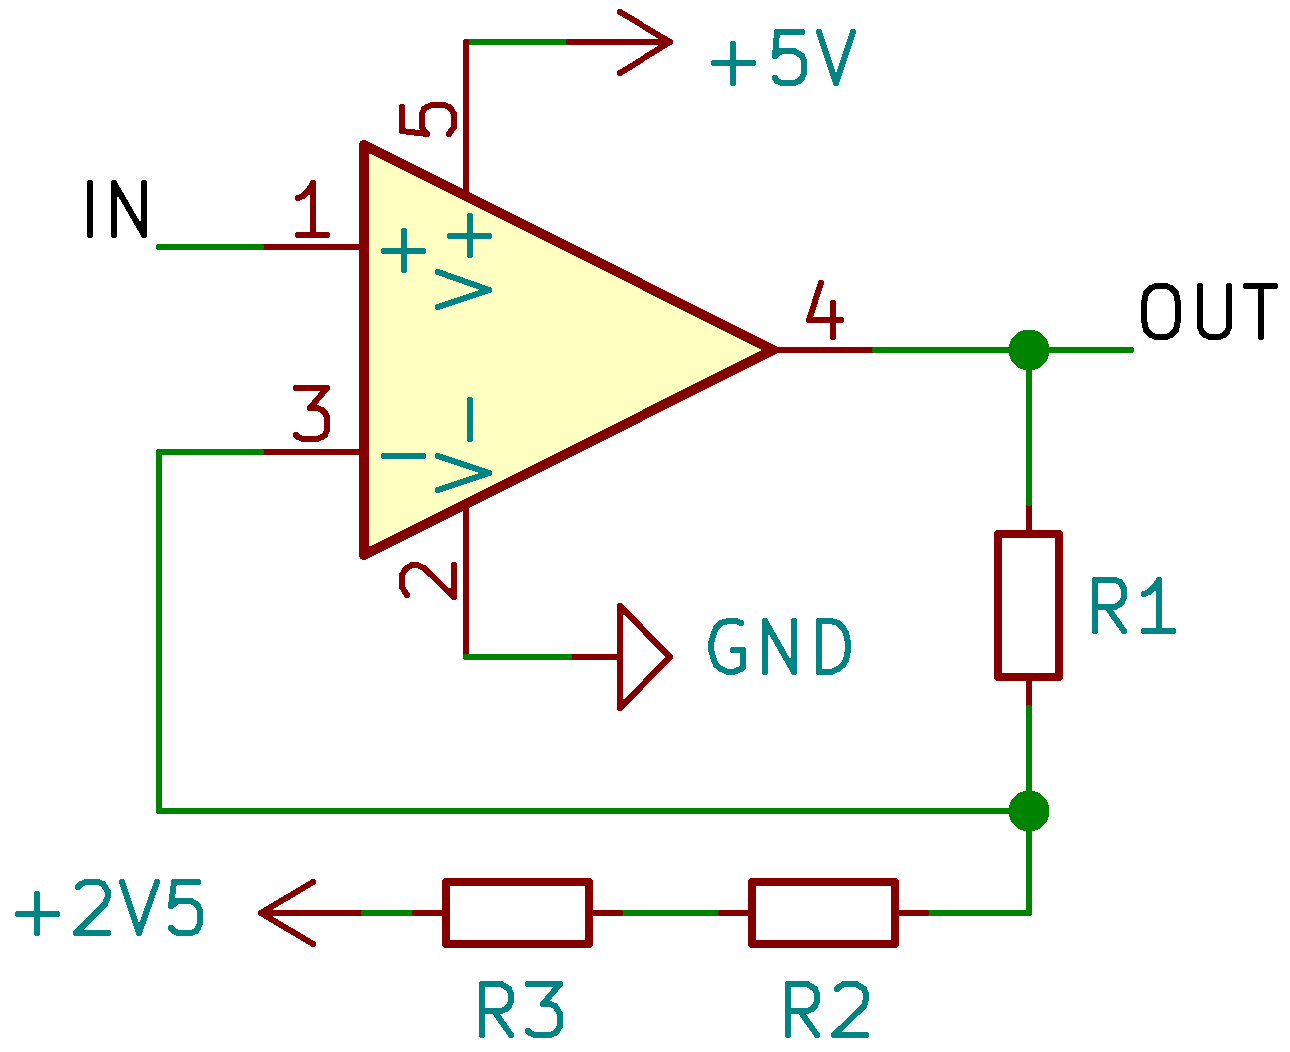
\includegraphics[width=0.3\textwidth]{gain_circuit}
	\caption{The non-inverting op-amp circuit.}
	\label{fig:non-inverting-op-amp}
\end{figure}

\begin{figure}[H]
	\centering
	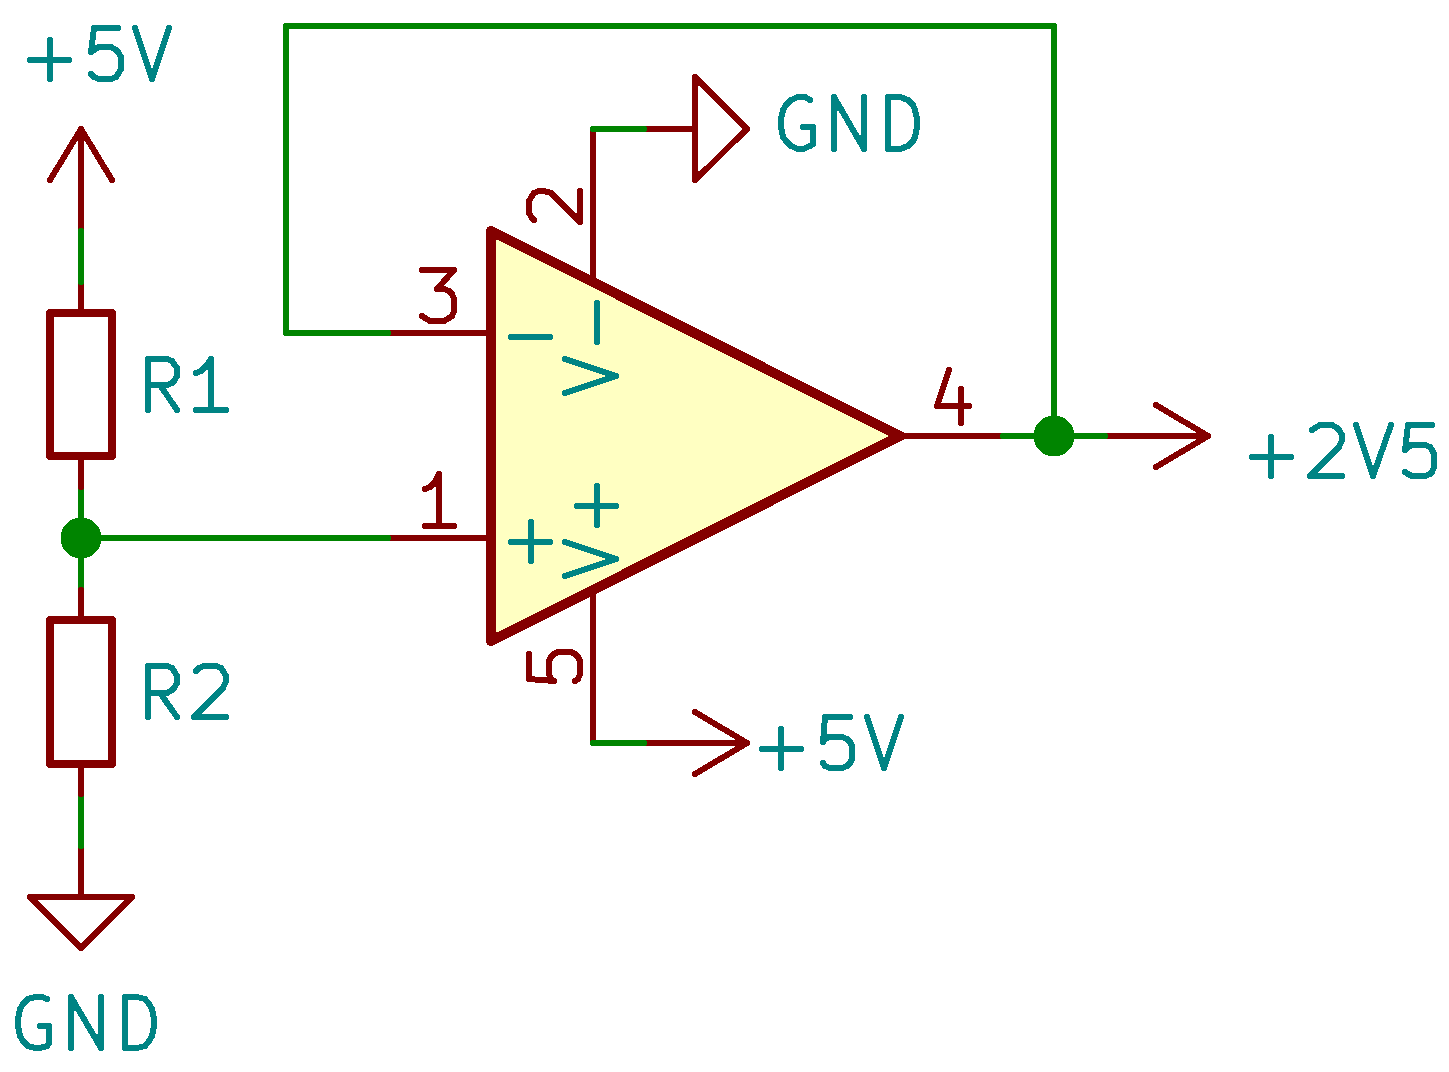
\includegraphics[width=0.3\textwidth]{virtual_ground_circuit}
	\caption{The virtual ground op-amp circuit.}
	\label{fig:half-supply}
\end{figure}

The op-amps are required to switch to a low power mode when no ADC readings are taking place.
Due to physical size constraints and part availability we have opted to disable the power supply to the op-amps to achieve a low power state.
The main drawback of this method is the start-up time to enable the op-amps.
The sum of the time taken to start the linear regulator and op-amp is less than $\SI{150}{\micro\second}$ (this is equivalent to $\SI{21.6}{\degree}$ of the $\SI{400}{\hertz}$ AC signal).

The source impedance is specified as being less than $\SI{100}{\ohm}$.
A input impedance that is an order of magnitude higher than the source impedance is required for maximum voltage transfer and minimum current drain.
$Z_i = \SI{1}{\kilo\ohm}$ was decided upon, because it is 10 times higher than the worst-case source impedance.
Equations \ref{eq:r1} and \ref{eq:r2} show the derived formulae for the resistors based upon the given $Z_i$ and $A$ values.
\begin{align}
	R_1 &= Z_i A \label{eq:r1} \\
	R_2 + R_3 &= \frac{Z_i A}{A - 1} \label{eq:r2} \\[1em]
	\therefore R_1 = \SI{100}{\kilo\ohm}, R_2 &= \SI{1}{\kilo\ohm}, R_3 = \SI{10}{\ohm} \nonumber
\end{align}

12 of these non-inverting amplifier circuits are required for each daughterboard.
The LMV324 selected as it has four op-amp circuits in one package, reducing the amount of space used on the board and the overall cost.
An additional package configured as unity gain amplifer produces the half-rail reference from a voltage divider input.
High value resistors are required in the divider (typically 100k$\omega$ to prevent excessive static current drain.
However these produce greater thermal noise, especially at high ambient temperatures, which is undesirable for ADC applications. Hence two 2k5$\omega$ balence nosie with 
static current drain of $\SI{1}{\milli\ampere}$

a 
Thermal calcuatins (not shown here for breitivy) show that the OpAmps will supply mimimal current into the microprocessor ADC inputs thus their power dissapation is reltively low.
Power dissabpatin is fiunction of the supply votage to ouput volateg diffence, ouput voalge diffenc to ground (for single suplkyt decies) and the ouput current.
With low power dissaption there is comfortable margin between the ambinent rempature of 105 degress, the gaurettened junction operting tempoate of 125 ddegress, and the device abolute maximu of 150 degrees.

Additnally worst case queincent current is 150uA.